\pdfoutput=1
\ifx\synctex\undefined\else\synctex=1\fi
\documentclass{llncs}


\usepackage[utf8]{inputenc}
\usepackage[T1]{fontenc}

\usepackage{microtype}

\usepackage{txfonts}
\let\iint\undefined 
\let\iiint\undefined 
\let\iiiint\undefined 
\let\idotsint\undefined 

\usepackage{amssymb}
\usepackage{mathtools} 

\usepackage{array}

\usepackage{tikz}
\usetikzlibrary{positioning}
\usetikzlibrary{arrows,automata}
\usetikzlibrary{calc}
\usetikzlibrary{decorations.pathreplacing}
\usetikzlibrary{matrix}
\usetikzlibrary{arrows}


\let\Asterisk\relax
\let\Note\relax
\usepackage[draft]{commenting}


\usepackage{paralist}

\usepackage[pdftex,colorlinks,hidelinks,
 	pdfauthor={Antoine Durand-Gasselin, Javier Esparza, Pierre Ganty, Rupak Majumdar},hypertexnames=false,pdftitle={Model Checking Parameterized Asynchronous Shared-Memory Systems}]{hyperref}


\makeatletter
\def\verbatim{\small\@verbatim \frenchspacing\@vobeyspaces \@xverbatim}
\makeatother

\newtheorem{notation}{Notation}{\itshape}{}

\newcommand{\Act}{{\cal A}}
\newcommand{\D}{{\cal D}}
\newcommand{\C}{{\cal C}}
\renewcommand{\S}{{\cal S}}
\newcommand{\G}{{\cal G}}
\newcommand{\N}{{\cal N}}
\newcommand{\betweenp}[1]{{\between}_{#1} }

\newcommand{\rb}{\ensuremath{r_{\star}}}
\newcommand{\wb}{\ensuremath{w_{\star}}}

\def\prod{\mathcal{P}}

\def\set#1{{\left\{ #1 \right\}}}
\def\tuple#1{{\left\langle #1 \right\rangle}}

\newcommand{\proj}{\mathit{Proj}}

\newcommand{\by}[1]{\xrightarrow{#1}}
\newcommand{\absby}[1]{\xrightarrow{#1}_\alpha}
\newcommand{\ds}[1]{{\it ds}(#1)}
\newcommand{\ap}[1]{{\it ap}(#1)}

\newcommand{\dom}{\textrm{dom}}

\renewcommand{\acute}[1]{\overrightarrow{#1}}
\renewcommand{\grave}[1]{\overleftarrow{#1}}


\sloppy

\setlength{\abovecaptionskip}{1ex}
\setlength{\belowcaptionskip}{1ex}
\setlength{\floatsep}{1ex}
\setlength{\textfloatsep}{1ex}

\declareauthor{rm}{Rupak}{blue}
\declareauthor{pg}{Pierre}{red}
\declareauthor{je}{Javier}{black!30!green}
\declareauthor{adg}{Antoine}{black!30!yellow}

\title{\texorpdfstring{Model Checking Parameterized Asynchronous Shared-Memory Systems}{Model Checking Parameterized Asynchronous Shared-Memory Systems}}
\author{Antoine Durand-Gasselin\inst{1} \and Javier Esparza\inst{1} \and Pierre Ganty\inst{2} \and Rupak Majumdar\inst{3}}
\institute{TU Munich \quad IMDEA Software Institute \quad MPI-SWS}

\pagestyle{plain}

\begin{document}

\maketitle

\begin{abstract}
\makeatletter{}

We characterize the complexity of liveness verification for
parameterized systems consisting of a leader process and arbitrarily many
anonymous and identical contributor processes.  Processes communicate through a shared,
bounded-value register. While each operation on the register is atomic, there
is no synchronization primitive to execute a sequence of operations atomically.



We analyze the case in which processes are
modeled by finite-state machines or pushdown machines and the property is given
by a B\"uchi automaton over the alphabet of read and write actions of the leader.
We show that the problem is decidable, and has a surprisingly low complexity: 
it is NP-complete when all processes are finite-state machines, and is PSPACE-hard and in NEXPTIME 
when they are pushdown machines. This complexity is lower than for the 
non-parameterized case: liveness verification of finitely many finite-state machines is 
PSPACE-complete, and undecidable for two pushdown machines. 

For finite-state machines, our proofs characterize infinite behaviors using existential abstraction
and semilinear constraints.
For pushdown machines, we show how contributor computations of high stack height can be simulated by computations of
many contributors, each with low stack height. 
Together, our results characterize the complexity of verification 
for parameterized systems under the assumptions of anonymity and asynchrony.


\end{abstract}

\makeatletter{}

\section{Introduction}

We study the verification problem for
\emph{parameterized asynchronous shared-memory systems} \cite{Hague11,egm13}. 
These systems consist of a \emph{leader} process and
arbitrarily many identical \emph{contributors}, processes with no identity, running at
arbitrary relative speeds.The shared-memory consists of a read/write register that all processes can access
to perform either a read operation or a write operation. The register is
bounded: the set of values that can be stored is finite. Read/write operations execute 
atomically but sequences of operations do not: no process can conduct an atomic sequence 
of reads and writes while excluding all other processes. 
In a previous paper \cite{egm13}, we have studied the complexity of safety verification, 
which asks to check if a safety property holds no matter how many contributors are present.
In a nutshell, we showed that the problem is coNP-complete when both leader and contributors
are finite-state automata and PSPACE-complete when they are pushdown automata.

In this paper we complete the study of this model by addressing the verification of liveness properties 
specified as -regular languages (which in particular encompasses LTL model-checking). 
Given a property like ``every request is eventually granted''
and a system with a fixed number of processes, one is often able to guess an upper bound
on the maximal number of steps until the request is granted, and replace the property
by the safety property ``every request is granted after at most  steps.'' 
In parameterized systems this bound can depend on the (unbounded) number of processes, and so 
reducing liveness to safety, or to finitary reasoning, is not obvious. 
Indeed, for many parameterized models, liveness verification is undecidable even if safety is decidable \cite{EFM99,rmeyer2008}.

Our results show that there is no large complexity gap between liveness and
safety verification: liveness verification (existence of an infinite computation
violating a property) is NP-complete in the finite-state
case, and PSPACE-hard and in NEXPTIME in the pushdown case.  
In contrast, remember that liveness checking is already PSPACE-complete for a {\em finite} number of finite-state
machines, and undecidable for a {\em fixed} number of pushdown systems.
Thus, not only is liveness verification decidable in the parameterized setting but 
the complexity of the parameterized problem is {\em lower} 
than in the non-parameterized case, where all processes are part of the
input. We interpret this as follows: in asynchronous shared-memory systems, the
existence of arbitrarily many processes leads to a ``noisy'' environment, in
which contributors may hinder progress by replying to past messages from the
leader, long after the computation has moved forward to a new phase. It is known
that imperfect communication  can {\em reduce} the power of computation and the complexity of verification
problems: the best known example are lossy channel systems, for which many verification
problems are decidable, while they are undecidable for perfect channels 
(see e.g. \cite{AbJo:lossy:IC,Parosh:etal:attractor:IC}). 
Our results reveal another instance of the same phenomenon.

Technically, our proof methods are very different from those used for safety
verification. 
Our previous results \cite{egm13} relied on a fundamental Simulation Lemma,
inspired by Hague's work \cite{Hague11}, stating that the {\em finite} behaviors of an arbitrary number of contributors can be simulated by a finite 
number of {\em simulators}, one for each possible value of the register. 
Unfortunately, the Simulation Lemma 
does not extend to infinite behaviors, and so we have to develop new ideas.
In the case in which both leader and contributors are finite-state machines, 
the NP-completeness
result is obtained by means of a combination of an abstraction
that overapproximates the set of possible infinite behaviors, and a semilinear constraint that
allows us to regain precision. The case in which both leader and contributors are 
pushdown machines is very involved. In a nutshell, we show that pushdown runs 
in which a parameter called the \emph{effective stack height} grows too much
can be ``distributed'' into a number of runs with smaller effective stack height.
We then prove that the behaviors of a pushdown machine with a bounded effective stack height 
can be simulated by an exponentially larger finite-state machine.

\noindent
\emph{Related Work.}
Parameterized verification has been studied extensively, both theoretically and practically.
While very simple variants of the problem are already undecidable \cite{AxKozen86}, 
many non-trivial parameterized models retain decidability.
There is no clear ``rule of thumb'' that allows one to predict what model checking 
problems are decidable, nor their complexities, other than ``liveness is generally harder than safety.''
For example, coverability for Petri nets---in which finite-state, identityless processes communicate via rendezvous or global shared state---
is EXPSPACE-complete, 
higher than the PSPACE-completeness of the non-parameterized version, and
verification of liveness properties can be equivalent to Petri net reachability, 
for which we only know non-primitive recursive upper bounds, or even undecidable.
Safety verification for extensions to Petri nets with reset or transfer, or broadcast protocols, where arbitrarily many finite-state processes communicate
through broadcast messages, 
are non-primitive recursive; liveness verification is undecidable in all cases \cite{ACJT96,EFM99,rmeyer2008}.
Thus, our results, which show simultaneously lower complexity than non-parameterized problems, as well as similar complexity for
liveness and safety, are quite unexpected.

German and Sistla \cite{GS92} and Aminof {\em et al.}~\cite{AminofKRSV14} 
have studied a parameterized model with rendezvous as communication primitive, where processes are 
finite-state machines. Model checking the fully symmetrical case---only contributors, no leaders---runs in 
polynomial time (other topologies have also been considered \cite{AminofKRSV14}),
while the asymmetric case with a leader is EXPSPACE-complete. 
In this paper we study the same problems, but for a shared memory communication primitive. 

\emph{Population protocols} \cite{Angluin} are another well-studied model of identityless 
asynchronous finite-state systems communicating via rendezvous. The semantics 
of population protocols is given over fair runs, in which every potential interaction that is infinitely often enabled is infinitely often taken. With this semantics, population protocols compute exactly the semilinear predicates \cite{Angluin}. In this paper we do not study what our model can compute (in particular, we are agnostic with respect to which fairness assumptions are reasonable),
but what we can compute or decide about the model. 

  






\makeatletter{}

\section{Formal Model: Non-Atomic Networks}
\label{sec:prelim}

In this paper, we identify systems with languages. System actions are
modeled as symbols in an alphabet, executions are modeled as infinite words,
and the system itself is modeled as the
language of its executions. Composition operations that combine systems into larger ones
are modeled as operations on languages.

\subsection{Systems as languages}An \emph{alphabet}  is a finite, non-empty set of \emph{symbols}. A
\emph{word} over  is a finite sequence over  including the
empty sequence denoted , and a \emph{language} is a set of
words. An \emph{-word} over  is an infinite sequence of
symbols of , and an \emph{-language} is a set of
-words.  We use  (resp.\  to denote the
language of all words (resp.\ -words) over .  When there is
no ambiguity, we use ``words'' to refer to words or -words.  We do
similarly for languages.  Let  be a sequence over some alphabet, define
 if  is a word; else (
is an -word)  denote the set .
Elements of  are called \emph{positions}.  The \emph{length} of a
sequence  is defined to be  and is denoted
.  We denote by  the symbol of  at position
 if ,  otherwise. Moreover, let
 with  and  denote . Also  denotes  For words , we
say  is a \emph{prefix} of  if either  or  and
there is a  such that .



\paragraph{Combining systems: Shuffle.} Intuitively, the shuffle of systems  and  is the system
interleaving the executions of  with those of . 
Given two -languages  and 
, their \emph{shuffle}, denoted by , 
is the -language over  defined as 
follows.
Given two -words , we say that  
is an \emph{interleaving} of  and  if there exist (possibly empty) words 
 and  such that 
each  is a prefix of ,
and each  is a prefix of ,
and  is an -word.
Then , where  denotes the set of all interleavings of  and
.  For  example, if  and , we get . 
Shuffle is associative and commutative, and so we can 
write  or .



\paragraph{Combining systems: Asynchronous product.} The asynchronous product of  and  also interleaves the executions but, this time,
the actions in the common alphabet must now be executed jointly.
The -language of the resulting system, called the \emph{asynchronous
product} of  and , is denoted by , and
defined as follows.  Let  be the word obtained by erasing
from  all occurrences of symbols not in .  is the -language over the alphabet
 such that  if{}f
 and  are prefixes of words in
 and , respectively. 
We abuse notation and write 
instead of  when .  For example, let
 and .  For 
and  we get . 
Observe that the language  depends on ,  and
also on  and . For example, if  and
, then , but if , then .  So we should more properly write
. However, since the alphabets
 and  will be clear from the context, we will omit
them. 
Like shuffle, asynchronous product is also associative and commutative, and so we write . Notice finally that
shuffle and asynchronous product coincide if , but usually differ otherwise. For instance, if  and , we get . 

We describe systems as combinations of shuffles and asynchronous products, for instance
we write . In these expressions we
assume that  binds tighter than , and so
 is the language ,
and not .


\subsection{Non-atomic networks}
\label{subsec:na-networks}
A non-atomic network is an infinite family of systems parameterized by a number
.  The th element of the family has  components communicating
through a global store by means of read and write actions.  The store is
modeled as an atomic register whose set of possible values is finite.  One
of the  components is the leader, while the other  are the
contributors. All contributors have exactly the same possible behaviors (they
are copies of the same -language), while the leader may behave
differently. The network is called non-atomic because components cannot
atomically execute sequences of actions, only one single read or write.

Formally, we fix a finite set  of \emph{global values}.
A {\em read-write alphabet} is any set of the form , where
 is a set of {\em read} and {\em write (actions)}. We denote a symbol
 by  and define .

We fix two languages  and
, called the \emph{leader} and the
\emph{contributor}, with alphabets  and
, respectively, where   are called
\emph{reads} and  are called \emph{writes}.   We write 
(respectively,  to stand for either  or  (respectively,
 or . We further assume that
 holds for every 
, else the value  is never used and can be removed from . 

Additionally, we fix an -language , called the {\em store}, 
over . It models
the sequences of read and write operations supported 
by an atomic register: a write  writes  to the register,
while a read  succeeds when the register's current value is . 
Initially the store is only willing to execute a write. 
Formally  is defined as 
 and any finite prefix thereof.
Observe that  is completely determined by  and .
Figure~\ref{fig:example} depicts a store with  as possible values as the language
of a transition system.

\begin{figure}[t]
\centering \noindent \begin{minipage}[c]{1.75cm}
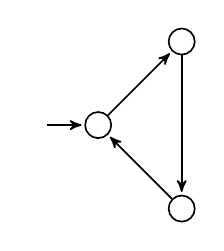
\begin{tikzpicture}[->,>=stealth',shorten >=1pt,auto,node distance=1.5cm, semithick]
\node[state,initial,initial text = {}, minimum size=2ex] (A) {};
\node[state,minimum size=2ex] (B) [above right of=A] {};
\node[state,minimum size=2ex] (C) [below right of=A] {};
\path[->] (A) edge node[left, font=\scriptsize] {} (B)
          (B) edge node[left, font=\scriptsize] {} (C)
          (C) edge node[left, font=\scriptsize] {} (A);
\end{tikzpicture}
\end{minipage}\hspace{\stretch{1}}\begin{minipage}[c]{5.5cm}
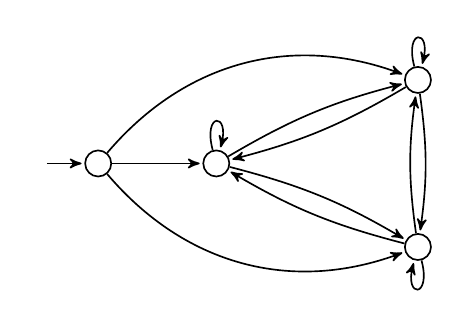
\begin{tikzpicture}[->,>=stealth',shorten >=1pt,auto,node distance=1.5cm, semithick]
\node[state,initial,initial text = {},minimum size=2ex] (A) {};
\node[state,minimum size=2ex] (B) [right of=A] {};
\node[state,minimum size=2ex] (C) [above right of=B, xshift=15mm] {};
\node[state,minimum size=2ex] (D) [below right of=B, xshift=15mm] {};

\path[->] (A) edge [bend left=35]  node[above, font=\scriptsize] {} (C) 
              edge node[above, font=\scriptsize] {} (B) 
              edge [bend right=35] node[below, font=\scriptsize] {} (D)
          (B) edge [loop above] node[above, font=\scriptsize] {} (B)
              edge [bend left=8] node[left,pos=0.7,yshift=1mm, font=\scriptsize]{} (C) 
              edge [bend left=8] node[right,pos=0.5,yshift=1mm, font=\scriptsize]{}(D) 
          (C) edge [loop above] node[left, font=\scriptsize] {} (C)
              edge [bend left=8] node[right,pos=0.5,yshift=-1mm, font=\scriptsize]{} (B) 
              edge [bend left=8] node[right, font=\scriptsize]{}(D)
          (D) edge [loop below] node[left, font=\scriptsize] {}(D)
              edge [bend left=8] node[left,yshift=-1mm, font=\scriptsize]{} (B) 
              edge [bend left=8] node[left,pos=0.5, font=\scriptsize]{}(C);
\end{tikzpicture}
\end{minipage}\hfill \begin{minipage}[c]{3.5cm}
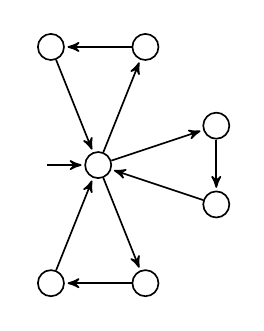
\begin{tikzpicture}[->,>=stealth',shorten >=1pt,auto,node distance=1.5cm, semithick]
\node[state,initial,initial text = {}, minimum size=2ex] (A) {};
\node[state,minimum size=2ex] (B) [above of=A, xshift= 6mm] {};
\node[state,minimum size=2ex] (C) [above of=A, xshift=-6mm] {};
\node[state,minimum size=2ex] (D) [right of=A, yshift=5mm] {};
\node[state,minimum size=2ex] (E) [right of=A, yshift=-5mm] {};
\node[state,minimum size=2ex] (F) [below of=A, xshift = 6mm] {};
\node[state,minimum size=2ex] (G) [below of=A, xshift = -6mm] {};

\path[->] (A) edge node[right,pos=0.65, font=\scriptsize] {} (B) 
              edge node[above, font=\scriptsize] {} (D) 
              edge node[right,pos=0.65, font=\scriptsize] {} (F)
          (B) edge node[above, font=\scriptsize] {} (C) 
          (C) edge node[left, font=\scriptsize] {} (A)
          (D) edge node[right, font=\scriptsize] {} (E) 
          (E) edge node[below, font=\scriptsize] {} (A)
          (F) edge node[below, font=\scriptsize] {} (G) 
          (G) edge node[left, font=\scriptsize] {} (A);
\end{tikzpicture}
\end{minipage}
\caption{Transition systems describing languages , , and .
We write .
The transition system for  is in state  when the current
value of the store is .} 
\label{fig:example}
\end{figure}
\begin{definition}\label{def:instancenetwork}
Let  and  be a leader and 
a contributor, and let . The \emph{-instance of the -network} 
is the -language \  \ where  
 stands for .
The {\em -network}  is the -language .
We omit the prefix  when it is clear from the context. 
It follows easily from the properties of shuffle and asynchronous product
that 
,
where  is an abbreviation of .
\end{definition}

Next we introduce a notion of {\em compatibility} between a word of the leader
and a multiset of words of the contributor (a multiset because 
several contributors may execute the same sequence of actions).  Intuitively, compatibility means
that all the words can be interleaved into a legal infinite sequence of reads
and writes supported by an atomic register---that is, an infinite sequence
belonging to . Formally:

\begin{definition}\label{def:CompRealReachpb}
Let , and let  be a multiset of words
over  (possibly containing multiple copies of a word).
We say that  is {\em compatible} with  if{}f the -language  is non-empty.
When  and  are compatible, there exists a word  such that .
We call  a \emph{witness} of compatibility.
\end{definition}

\begin{example}
Consider the network with  where the leader, store, and
contributor languages are given by the infinite paths of the
transition systems from Figure~\ref{fig:example}. The only
-word of  is  and the
-language of  is
. For
instance,  is compatible with the
multiset  of  -words obtained by taking two copies 
of ,  and .
The reader may be interested in finding another multiset compatible with  and containing
only 4 -words.
\end{example}

\paragraph{Stuttering property.}
Intuitively, the stuttering property states that if 
we take an -word of a network  and ``stutter'' reads and writes
of the contributors, going e.g. from 
to , the result
is again an -word of the network.

Let  be a witness of compatibility of 
and . Pick a set  of positions (viz.  such that  for each ,
and pick a number  for every .  Let  be the result of simultaneously 
replacing each  by  in . We have that . 
Now let , where ,  , 
It is easy to see that  , 
and so  is compatible with , the multiset consisting of  and , 
and  is a witness of compatibility.

An easy consequence of the stuttering property is the \emph{copycat lemma}~\cite{egm13}.
\begin{lemma}[Copycat Lemma]
\label{lem:extendedmono}
Let  and let  be a multiset of words of
.  If  is compatible with , then  is also compatible with 
for every .
\end{lemma}

\subsection{The Model-checking Problem for Linear-time Properties} 

We consider the model checking problem for linear-time properties, 
that asks, given a network  and an -regular language
, decide whether  is non-empty.
We assume  is given as a B\"uchi automaton  over .
Intuitively,  is a tester that observes the actions of the leader;
we call this the \emph{leader model checking problem}.


We study the complexity of leader model checking for networks in which the 
read-write -languages  and  of leader and contributor are generated by 
an abstract machine, like a finite-state machine (FSM) or a pushdown machine (PDM). 
(We give formal  definitions later.) 
More precisely, given two classes of machines \texttt{D}, \texttt{C}, 
we study the model checking problem  defined as follows: 
\begin{compactdesc}
\item[{\bf Given}:] machines  and , 
and a B\"uchi automaton  
\item[{\bf Decide}:] Is  non-empty? 
\end{compactdesc}

In the next sections we prove that 
and  are NP-complete, 
while  is in NEXPTIME and PSPACE-hard. 

\begin{example}
Consider the instance of the model checking problem where  and  are as in Figure~\ref{fig:example},
and  is a B\"uchi automaton recognizing all words over  containing infinitely many 
occurrences of . Since  is compatible with a multiset of words of the contributors, 
 is non-empty. In particular, .
\end{example}

Since , we can replace  and  by a
machine  with a B\"uchi acceptance condition. The construction
of  given  and  is standard.
In what follows, we assume that  comes with a B\"uchi acceptance condition and forget about .

There are two natural variants of the model checking problem, where , i.e., the alphabet of  contains the actions of all
contributors, or .  In both these
variants, the automaton A can be used to simulate atomic networks.  Indeed, if
the language of A consists of all sequences of the form , and we design the contributors so that they alternate reads
and writes, then the accepting executions are those in which the contributors
read a value from the store and write a new value in an atomic step. So the
complexity of the model-checking problem coincides with the complexity for
atomic networks (undecidable for PDMs and EXPSPACE-complete for FSMs), and we
do not study it further.



\makeatletter{}

\section{ is NP-complete}
\label{sec:fsafsa}

We fix some notations. A finite-state machine (FSM)  over  consists of a
finite set of states  containing an initial state  and a transition
relation .
A word  is \emph{accepted} by an
FSM if there exists a
sequence  of states such that
 for all . We denote by  the \emph{run} accepting .  
A B\"uchi automaton  is an FSM  
together with a set  of accepting
states. An -word  is accepted by a B\"uchi automaton if there is a run  such that   for infinitely many positions .
The -language of a FSM or B\"uchi automaton , denoted by , is the set of -words accepted by .

In the rest of the section we show that  is NP-complete. 
Section \ref{subsec:TS} defines the infinite
transition system associated to a (\texttt{FSM},\texttt{FSM})-network. Section \ref{subsec:absTS} introduces
an associated finite abstract transition system. Section \ref{subsec:realiz} states and proves 
a lemma (Lemma \ref{lem:realizability}) characterizing the cycles of the
abstract transition system that, loosely speaking, can be concretized into
infinite executions of the concrete transition system. Membership in NP is then proved using the lemma. 
NP-hardness follows from NP-hardness of
reachability~\cite{egm13}. 


\subsection{(\texttt{FSM},\texttt{FSM})-networks: Populations and transition system} 
\label{subsec:TS} 
We fix a B\"uchi automaton  over  and an FSM  
over . A {\em configuration} 
is a tuple , where , , and  
assigns to each state of  a natural number. Intuitively,  
is the current state of ;  is a value or the special value , 
modelling that the store has not been initialized yet, and no process
read before some process writes; finally,  is the number of contributors 
currently at state . We call  a {\em population} of , and write  for
the {\em size} of . Linear combinations
of populations are defined componentwise: for every
state , we have . Further, given , we denote by  the population
 if  and  otherwise,
i.e., the population with one contributor in state  and no contributors elsewhere.
A configuration is \emph{accepting} if the state of  is accepting, that is whenever .
Given a set of populations , we define 
. 

The labelled transition system  associated to  is defined
as follows:  
\begin{compactitem}
\item  is the set of all configurations, and  is
 the set of initial configurations, given by , where ;
\item , where
  \begin{compactitem}
  \item  is the set of triples 
  such that  is a transition of , viz. , and one of the following conditions holds:
  \begin{inparaenum}[(i)]
  \item ; or
  \item , .
  \end{inparaenum}
  \item  is the set of triples 
  \noindent such that , and one of the following conditions holds:
  \begin{inparaenum}
  \item[(iii)] , , and 
  ; or
  \item[(iv)] , , , 
  and .
  \end{inparaenum}
  \end{compactitem}
  Observe that ,
  because the total number of contributors  of a population remains constant.
Given configurations  and , 
we write  if . 
  \end{compactitem}
We introduce a notation important for Lemma \ref{lem:realizability} below.
We define . 
Observe that
 in cases (i) and (ii) above, and  
in cases (iii) and (iv). So  depends only on the transition ,
but not on .  
\subsection{The abstract transition system} 
\label{subsec:absTS} 
We introduce an {\em abstraction function}  that assigns to a set  of populations
the set of states of  populated by . We also introduce a
{\em concretization function}  that assigns to a set  the set of  
all populations  that only populate states of . Formally:
{
\setlength\abovedisplayskip{1pt}
\setlength\belowdisplayskip{1pt}

}
\noindent It is easy to see that  and  satisfy  
and , and so  and  form a Galois connection 
(actually, a Galois insertion). 
An {\em abstract configuration} is a tuple , where , , and . 
We extend  and  to (abstract) configurations in the obvious way.
An abstract configuration is \emph{accepting} when the state of  is accepting, that is whenever .

Given , we define its  {\em abstraction} 
 as follows: 
\begin{compactitem}
\item  is the set of all abstract configurations.
\item 
is the initial configuration.
\item  if{}f
there is  and  such that \\ 
 and
.
\end{compactitem}
Observe that the number of abstract configurations 
is bounded by . 
Let us point out that our abstract transition system resembles but is different from that of Pnueli et al.\cite{PnueliXZ02}.
We write  if . 
The abstraction satisfies the following properties:
\begin{compactitem}
\item[(A)] For each -path  of , 
there exists an -path
 in  such that 
 for all .
\item[(B)] If , then . \\
To prove this claim, consider two cases:
\begin{compactitem}
\item . Then 
for every population  (because only the leader moves). So 
. 
\item . Consider the population 
. Then 
, where 
. But 
then , and so 
, which implies 

for some . 
\end{compactitem}
\end{compactitem}
\noindent So in every -path  
of , where , there is an index
 at which the  stabilize, that is,   holds for every .
However, the converse of (A) does not hold: given a path
 of , there may
be no path  in  such that
 for every . 
Consider a contributor machine  with two states  and one single transition
. Then  contains the infinite path (omitting the 
state of the leader, which plays no role):
{
\setlength\abovedisplayskip{1pt}
\setlength\belowdisplayskip{1pt}

}
\noindent 
However, the transitions of  are of the form
, 
and so  has no infinite paths.

\subsection{Realizable cycles of the abstract transition system} 
\label{subsec:realiz}
We show that the existence of an infinite accepting path in 
reduces to the existence of a certain lasso path in .  A
lasso path consists of a stem and a cycle.  
Lemma~\ref{lem:cover} shows
how every abstract finite path (like the stem) has a counterpart in .
Lemma~\ref{lem:realizability}
characterizes precisely those cycles in  which have an
infinite path counterpart in . 

\begin{lemma}
	Let  be an abstract configuration of  reachable from 
	 (.
	For every , there exists  such that
	 is reachable from 
	and .
	\label{lem:cover}
\end{lemma}
Lemma~\ref{lem:cover} does not hold for atomic networks. Indeed, consider a contributor
with transitions , where 
 denotes that the read and the write happen in one single atomic step.
Then we have (omitting the state of the leader, which does not play any r\^ole here):
{
\setlength\abovedisplayskip{1pt}
\setlength\belowdisplayskip{1pt}

}
\noindent 
Let  be the population putting one contributor in each of 
. This population belongs to 
but no configuration  with
 is reachable from any population that only puts 
contributors in , no matter how many. Indeed, after the first contributor
moves to , no further contributor can follow, and so we cannot have contributors
simultaneously in both  and . On the contrary, in non-atomic networks 
the Copycat Lemma states that what the move by one 
contributor can always be replicated by arbitrarily many.

We proceed to characterized the cycles of the abstract transition system that can be
``concretized''. A {\em cycle} of  is a path 

such that . A cycle is {\em realizable} if there is an
infinite path  of  such that 
 and  for every .

\begin{lemma}\label{lem:realizability}
A cycle  of 
 is realizable if{}f .
\end{lemma}


\begin{theorem}
\label{th:fsafsa}
 is NP-complete.
\end{theorem}
\begin{proof}
NP-hardness
follows from the NP-hardness of reachability \cite{egm13}.
We show membership in NP with the following high-level 
nondeterministic algorithm whose correctness 
relies on Lemmas~\ref{lem:cover} and \ref{lem:realizability}:
\begin{enumerate}
	\item Guess a sequence  of subsets of  such that  for all , . Note that .
	\item Compute the set  of abstract configurations and the set  of abstract transitions 
	      between configurations of .
	\item Guess an accepting abstract configuration , that is, an
  such that  is accepting in .
	\item Check that  is reachable from the initial abstract configuration  by means of abstract transitions of . 
	\item Check that the transition system with  and 
as states and transitions contains a cycle 
such that ,  and .
\end{enumerate}
We show that the algorithm runs in polynomial time. First, because the sequence guessed is no longer 
than , the guess can be done in polynomial time. 
Next, we give a polynomial algorithm for step (5):
\begin{compactitem}
\item Compute an FSA\footnote{A finite-state automaton (FSA) is an FSM which decides languages of finite words. Therefore an FSA is an FSM with a set  of accepting states.}  over the alphabet
		 with  as set of states,
		 as set of transitions,  as initial state, and  
                 as set of final states.
	\item Use the polynomial construction of Seidl \textit{et al.}~\cite{Seidl05} to compute an (existential) Presburger formula  for the Parikh
		image of . 
		The free variables of  are in one-to-one correspondence with the transitions of . Denote by 
		the variable corresponding to transition .
	\item Compute the formula 
		{
\setlength\abovedisplayskip{1pt}
\setlength\belowdisplayskip{1pt}
		
		}
\noindent where  and  returns the target and source states of the transition passed in argument.  adds to  the realizability condition of Lemma \ref{lem:realizability}.
	\item Check satisfiability of . This step requires nondterministic polynomial 
              time because satisfiability of an existential Presburger formula is in NP \cite{Gradel88}.\qed
\end{compactitem}
\end{proof}



\makeatletter{}


\section{ is NP-complete}
\label{sec:pdafsa}

A pushdown system (PDM)  over  consists of a finite set  of states 
including the initial state ,
a \emph{stack alphabet}  including the bottom stack symbol , and a set of \emph{rules}
 which either push or pop as explained below.
A \emph{PDM-configuration}  consists of a state  and a word
 (denoting the stack content).  For , , , , we say a
PDM-configuration  (resp. ) -follows  if ,
(resp. ); we write  if  -follows , and call it a {\em transition}.
A \emph{run}  on a word 
is a sequence of PDM-configurations such that  and 
 for all .
We write  if there is a run from  to . 
The language  of  is the set of all words 
such that  has a run on .

A B\"uchi PDM is a PDM with a set  of accepting states.
A word is accepted by a B\"uchi PDM if there is a run on the word for which some state in  occurs infinitely often along the
PDM-configurations. The following lemma characterizes accepting runs.

\begin{lemma}{\cite{BEM97}}
\label{lem:pdacycle}
Let  be a configuration.
There is an accepting run starting from  if there are states , ,
a stack symbol  such that
 for some 
and  for some .
\end{lemma}

We now show  is decidable, generalizing the proof from Section~\ref{sec:fsafsa}.
Fix a B\"uchi PDM , and a FSM . 
A {\em configuration} is a tuple , where ,
 is the stack content, , and  is a population.
Intuitively,  is the PDM-configuration of the leader.
We extend the definitions from Section~\ref{sec:fsafsa} like accepting configuration in the obvious way.

We define a labeled transition system , where  is the set of configurations including the set  of initial configurations,
and the transition relation , where  is as before and  is the set of triples
 
  such that  is a transition (not a rule) of , and one of the following conditions holds:
  \begin{inparaenum}[(i)]
  \item ; or
  \item  and .
  \end{inparaenum}
We define the abstraction  of  as the obvious generalization of the abstraction in Section~\ref{sec:fsafsa}.
An accepting path of the (abstract) transition system is an infinite path  with infinitely many accepting (abstract) configurations. As for , not every accepting path of the abstract admits a concretization, but we find a realizability condition in terms of linear constraints. Here we use again the polynomial construction of 
Seidl \textit{et al.}~\cite{Seidl05} mentioned in the proof of 
Theorem \ref{th:fsafsa}, this time to compute an (existential) Presburger formula
for the Parikh image of a pushdown automaton. 



\begin{theorem}
\label{th:pdafsa}
 is NP-complete.
\end{theorem}




\makeatletter{}

\section{ is in NEXPTIME}
\label{sec:pdapda}

We show how to reduce  to
.
We first introduce the notion of {\em effective stack height} of a 
PDM-configuration in a run of a PDM, and define, given a PDM ,  
an FSM  that simulates all the runs of  of effective stack height .
Then we show that, for , where  is the size of ,
the language  is
empty if{}f  
is empty. 


\subsection{A FSM for runs of bounded effective stack height}

Consider a run of a PDM that repeatedly pushes symbol on the
stack. The stack height of the configurations\footnote{
For readability, we write ``configuration'' for ``PDM-configuration.''
}
 is unbounded, but,
intuitively, the PDM only uses the topmost stack symbol during
the run. To account for this we define the notion of effective stack height.

\begin{definition}
  Let  be an infinite run of a
  PDM on -word , where . 
The {\em dark suffix} of  in , denoted by , is
  the longest suffix of  that is also a proper suffix of  for
  every . The {\em active prefix}  of  is the
  prefix satisfying .
The {\em effective stack height} of  in  is 
	.
We say that  is {\em effectively -bounded} (or simply -bounded
	for the sake of readability) if every configuration of  has an
	effective stack height of at most . 
Further, we say that  is {\em bounded} if it is -bounded for some .  Finally, an -word of the PDM is {\em -bounded},
	respectively bounded, if it is the word generated by some -bounded,
	respectively bounded, run (other runs for the same word may not be bounded).
\end{definition}

Intuitively, the effective stack height measures the actual memory required by
the PDM to perform its run. 
For example, repeatedly pushing symbols on the stack produces a run with
effective stack height 1.  
Given a position in the run, the elements of the stack that are never popped
are those in the longest common suffix of all subsequent stacks.
The first element of that suffix may be read, therefore only the
longest \emph{proper} suffix is effectively useless, so  
no configuration along an infinite run has effective stack height . 


\begin{proposition}\label{prop:esh1often}
Every infinite run of a PDM contains infinitely many positions at which the
effective stack height is 1.
\end{proposition}
 \begin{proof}
 Let  be any infinite run. 
 Notice that  for every , because otherwise the run would not
 be infinite. Let  be the set of positions of the run defined as:
  if{}f  for every . Observe that
  is infinite, because the first configuration of minimal stack height,
 say  belongs to it, and so does the first configuration of minimal stack height
 of the suffix , etc.
 By construction, the configuration at every position in  has effective stack height .\qed
 \end{proof}

In a -bounded run, whenever
the stack height exceeds , the -th stack symbol will never become the top symbol
again, and so it becomes useless. 
So, we can construct a finite-state machine  recognizing the words of 
accepted by -bounded runs. 

\begin{definition}
  Given a PDM , the FSM ,
	called the \emph{-restriction of }, is defined as follows: (a)  (a state of  consists of a state of  and a stack content no longer than );
(b) q w \by{a} q' w'D \label{eq:reduction} \big(L(D) \parallel \S \parallel \betweenp{\infty} L(C)\big) \neq
	\emptyset \quad\text{if{}f}\quad \big(L(D) \parallel \S \parallel 
	\betweenp{\infty} L(C_N)\big) \neq \emptyset \enspace .\tag{} \dom(\rho) (\rho)_k (\rho)_{i..j} (\rho)_{i..\infty} (\rho')_i = (\rho)_{\psi(\rho',i)}\rho = r_ar_br_br_cr_cr_cR = \{\rho'_1, \rho'_2, \rho'_3\}\psiS = \{\sigma'_1, \sigma'_2, \sigma'_3\}\psi'\begin{array}{r|ccc}
\psi    &  1  &  2  &  3   \\ \hline
\rho'_1 &  1  &  6  &      \\
\rho'_2 &  1  &  2  &  5   \\
\rho'_3 &  1  &  3  &  4
\end{array}\begin{array}{rccccccc}
        &   &   1  &  2  &  3  &  4  &  5  & 6  \\ \hline
\rho    & = &  r_a & r_b & r_b & r_c & r_c & r_c\\
\rho'_1 & = &  r_a &     &     &     &     & r_c\\
\rho'_2 & = &  r_a & r_b &     &     & r_c &    \\
\rho'_3 & = &  r_a &     & r_b & r_c &     &    
\end{array}\begin{array}{r|ccccccc}
\psi'     &  1  &  2  &  3  &  4  \\ \hline
\sigma'_1 &  1  &  4  &     &     \\
\sigma'_2 &  1  &  2  &  4  &  5  \\
\sigma'_3 &  1  &  3  &  5  &  6
\end{array}\begin{array}{rccccccc}
          &   &   1  &  2  &  3  &  4  &  5  & 6  \\ \hline
\rho      & = &  r_a & r_b & r_b & r_c & r_c & r_c\\
\sigma'_1 & = &  r_a &     &     & r_c &     &    \\
\sigma'_2 & = &  r_a & r_b &     & r_c & r_c &    \\
\sigma'_3 & = &  r_a &     & r_b &     & r_c & r_c   
\end{array}\rho)_{2..4}\rho'_2)_2
(\rho'_3)_{2..3}k \in\dom(\rho')c_\psi(\rho',k) = c(\rho', {\it last}_{\psi}(\rho', k))r_a,r_br_cc_\psi(\rho', i) = c(\rho,i)\{ \acute{p}_1, \grave{p}_1, \acute{p}_2, \grave{p}_2, \ldots, \acute{p}_N, \grave{p}_N\} \subseteq \dom(\rho) i1\leq i\leq Nc(\rho,\acute{p}_i)c(\rho,\grave{p}_i)\acute{p}_i\grave{p}_iw_p \alpha_i \alpha_{i-1} \cdots \alpha_1 w_0w_p \in
\Gamma_C^*c(\rho,\acute{p}_i)	= q_i \alpha_i \alpha_{i-1} \ldots \alpha_0 w_0c(\rho,\grave{p}_i)	= q'_i \alpha_{i-1} \ldots \alpha_0 w_0q_i, q'_i\in Q_C\acute{p}_1 < \cdots < \acute{p}_{N-1} < \acute{p}_N < Z < \grave{p}_N < \grave{p}_{N-1} < \cdots < \grave{p}_1
	\rho =  (\rho)_{1..\acute{p}_{j_1}} 
\ [q\alpha w_1]\ 
(\rho)_{\acute{p}_{j_1+1}..\acute{p}_{j_2}}
\ [q\alpha w_2 w_1]\ 
(\rho)_{\acute{p}_{j_2+1}..\acute{p}_{j_3}}
\ [q\alpha w_3 w_2 w_1] \\
(\rho)_{\acute{p}_{j_3+1}..\grave{p}_{j_3}}
\ [q'w_3 w_2 w_1]\ 
(\rho)_{\grave{p}_{j_3+1}..\grave{p}_{j_2}}
\ [q' w_2 w_1]\ 
(\rho)_{\grave{p}_{j_2+1}..\grave{p}_{j_1}}
\ [q' w_1]\ 
(\rho)_{\grave{p}_{j_1+1}..\infty}\enspace .
\rho_a\rho (\rho)_{\acute{p}_{j_1+1}..\acute{p}_{j_2}} (\rho)_{\grave{p}_{j_2+1}..\grave{p}_{j_1}}\rho_b (\rho)_{\acute{p}_{j_2+1}..\acute{p}_{j_3}} (\rho)_{\grave{p}_{j_3+1}..\grave{p}_{j_2}}\rho_a (\rho)_{1..\acute{p}_{j_1}} 
\ [q\alpha w_1]\ 
(\rho)_{\acute{p}_{j_2+1}..\acute{p}_{j_3}}
\ [q\alpha w_3 w_1] \\
(\rho)_{\acute{p}_{j_3+1}..\grave{p}_{j_3}}
\ [q' w_3 w_1]\ 
(\rho)_{\grave{p}_{j_3+1}..\grave{p}_{j_2}}
\ [q' w_1]\ 
(\rho)_{\grave{p}_{j_1+1}..\infty}\enspace .\rho_b\pi \in \S\pi \in \sigma
\between \rho \lambda_1 [\lambda_2]^{\omega} p\pip_{\sigma}\sigma (\sigma)_{1..p_\sigma} = \proj_{\Sigma_{\D}}( (\pi)_{1..p})p_\rho\rho)_{1..p_\rho} = \proj_{\Sigma_{\C}}((\pi)_{1..p})c(\sigma,i_\sigma) c(\sigma,k_\sigma){\alpha}{\it TS}{\alpha}X_0 = ( q_{0D}, \#, \alpha(\vec{P_0}))= ( q_{0D}, \#, \{q_{0C}\}) (q_D,g,Q) q_D,g,Q) = ( q_{0D}, \#,
	\{q_{0C}\})n > 0 ( q_{1D}, g_1, Q_1) \absby{t} ( q_D, g, Q)t\in T_Ct\in T_DQ_1 = Qq_C{q_C}'t\absby{}
		Q = \alpha\left( \, \left\{ \vec{p'} \mid \exists \vec{p}\in \gamma(Q_1) \colon \vec{p} \geq \vec{q_C} \land \vec{p'} = \vec{p} - \vec{q_C} + \vec{q_C}' \right\} \, \right)\enspace .	
		\label{eq:Q}
	Q = Q_1 \cup \{ {q_C}' \} Q_1 = Q\vec{p}\in \gamma(Q)d = \vec{p}({q_C}')\vec{p_1} = \vec{p} - d \vec{q_C}' + d \vec{q_C}\vec{p_1}(q_C') = d - d = 0\vec{p_1} \in \gamma(Q_1)\vec{\hat{p}_1} \in
	\gamma(Q_1)\vec{\hat{p}_1} \geq \vec{p_1} q_{1D}, g_1,\vec{\hat{p}_1})X_0{\it TS}\vec{\hat{p}_1} \geq \vec{p_1} \geq d\vec{q_C}\vec{\hat{p}} = \vec{\hat{p}_1} - d\vec{q_C} + d\vec{q_C}'dt \in \delta_C  (q_{1D}, g_1, \vec{\hat{p}_1}) \by{t^d} (q_D, g,
	\vec{\hat{p}_1} - d\vec{q_C} + d\vec{q_C}') = (q_D, g, \vec{\hat{p}}) c_0 \in \gamma(a_0), \ldots, c_{n-1}\in\gamma(a_{n-1})c_k \in \gamma(a_{(k\mod n)})
\vec{p}_{k_2 n} = \vec{p}_{k_1 n} + \sum_{i=(k_1 n) +1}^{k_2 n} \Delta(t_i) \enspace ,
\shortintertext{the sum on the right-hand-side is equal to . Since}
\sum_{i=(k_1 n) +1}^{k_2 n} \Delta(t_i) = (k_2 - k_1) \sum_{i=1}^{n} \Delta(t_i)
{\it TS}\alpha{\it TS} ( q_{0D}, \#, \vec{P_0}) {\it TS}i_1 < i_2c_{i_1} = c_{i_2}\sum_{k=i_1}^{i_2} \Delta(t_i) = \vec{0}\omega\alpha{\it TS}\omega\alpha{\it TS}c_i \in \gamma(a_i)i\geq 0DAc_ia_iii\geq 0Q_i \subseteq Q_{i+1}D\DC\C (\D,\C)\Nw_d(\)\D\omegar_d(\)\D\CCFw_c(\#)Q_1,\ldots,Q_{\ell}Q_CQ_i \subsetneq Q_{i+1}i0 < i < \ell \leq \vert{Q_C}\vert Q_D \times (\G\cup\{\#\}) \times \{ \{q_{0C}\} , Q_1,\ldots,Q_{\ell} \} FP^{\circlearrowright}_{q\gamma}P^{\circlearrowright}_{q\gamma}\OmegaL(P^{\circlearrowright}_{q\gamma})\Omegax_tt\in \delta_D\cup\delta_C\Omega'\vert{Q_C}\vert\vert{Q_C}\vertq_c\in Q_C\sum_{\mathrm{tgt}(t) =
q_c} x_t = \sum_{\mathrm{src}(t) = q_c} x_t \mathrm{tgt}\mathrm{src}\sum_{t\in \delta_D\cup \delta_C} x_t > 0\vec{0}\Omega'q_i, \ap{i}u_i)\vert{\ap{i+1}u_{i+1}}\vert\leq kq_i, \ap{i} u_i) \by{(v)_{i+1}} (q_{i+1}, \gamma \ap{i} u_i)\vert{\ap{i+1} u_{i+1}}\vert \leq kq_i, \ap{i} u_i) \by{(v)_{i+1}} (q_{i+1}, \ap{i+1} u_{i+1})P_k\vert{\gamma \ap{i} u_i}\vert = k+1\vert{\ap{i}}\vert=k\vert{\ap{i+1} u_{i+1}}\vert \leq kq_i, \ap{i} u_i) \by{(v)_{i+1}} (q_{i+1}, \ap{i+1} u_{i+1})P_k
  \label{eq:inv}
	|w_{i+1}w'_{i+1}| - |w_iw'_i| \geq |w_{i+1}| - |w_i|, \quad\text{for all } i\geq 0\enspace .
  \vert{w_{i+j}w'_{i+j}}\vert
  - \vert{w_iw'_i}\vert \geq \vert{w_{i+j}}\vert -
  \vert{w_i}\vertr_a,r_br_c\begin{array}{r|cccccccccc}
               &    &  0       &  1                &  2                   &  3                         &  4                    &  5             &  6    \\ \hline
\rho \colon    & \; & \; \bot \;  &  \; \alpha \bot \;   & \; \alpha\alpha\bot \;  & \; \alpha\alpha\alpha\bot \;  & \; \alpha\alpha\bot \;   & \; \alpha\bot \;  & \; \bot \; \\
{\it e.s.h.}   &    &  1       &  2                &  3                   &  4                         &  3                    &  2             &  1    \\ \hline
\rho'_1 \colon &    &  \bot    &  \alpha\bot       &                      &                            &                       &                & \bot \\
{\it e.s.h.}   &    &  1       &  2                &                      &                            &                       &                & 1     \\ \hline
\rho'_2 \colon &    &  \bot    &  \alpha\bot       &  \alpha\alpha\bot    &                            &                       &  \alpha\bot    &       \\
{\it e.s.h.}   &    &  1       &  1                &  2                   &                            &                       &  1             &       \\ \hline
\rho'_3 \colon &    &  \bot    &  \alpha\bot       &                      &  \alpha\alpha\bot          &  \alpha\bot           &                &       \\
{\it e.s.h.}   &    &  1       &  1                &                      &  2                         &   1                   &                &       \\ \hline
\end{array}
\qquad 
\begin{array}{r|cccccccccc}
                 &    &  0       &  1                &  2                   &  3                         &  4                    &  5             &  6    \\ \hline
\rho \colon      & \; & \; \bot \;  &  \; \alpha \bot \;   & \; \alpha\alpha\bot \;  & \; \alpha\alpha\alpha\bot \;  & \; \alpha\alpha\bot \;   & \; \alpha\bot \;  & \; \bot \; \\
{\it e.s.h.}     &    &  1       &  2                &  3                   &  4                         &  3                    &  2             &  1    \\ \hline
\sigma'_1 \colon &    &  \bot    &  \alpha\bot       &                      &                            &  \bot                 &                &       \\
{\it e.s.h.}     &    &  1       &  2                &                      &                            &  1                    &                &       \\ \hline
\sigma'_2 \colon &    &  \bot    &  \alpha\bot       &  \alpha\alpha\bot    &                            &  \alpha\bot           &  \bot          &       \\
{\it e.s.h.}     &    &  1       &  2                &  3                   &                            &  2                    &  1             &       \\ \hline
\sigma'_3 \colon &    &  \bot    &  \alpha\bot       &                      &  \alpha\alpha\bot          &                       & \alpha\bot     & \bot  \\
{\it e.s.h.}     &    &  1       &  2                &                      &  3                         &                       & 2              & 1     \\ \hline
\end{array}
{\it last}_\psi(\sigma'_i,0){\it last}_\psi(\sigma'_i,6)\rho\{ \acute{p}_1, \grave{p}_1, \acute{p}_2, \grave{p}_2, \ldots, \acute{p}_N, \grave{p}_N\} \subseteq \dom(\rho) i1\leq i\leq Nc(\rho,\acute{p}_i)c(\rho,\grave{p}_i)\acute{p}_i\grave{p}_iw_p \alpha_i \alpha_{i-1} \cdots \alpha_1 w_0w_p \in
\Gamma_C^*c(\rho,\acute{p}_i)	= q_i \alpha_i \alpha_{i-1} \ldots \alpha_0 w_0c(\rho,\grave{p}_i)	= q'_i \alpha_{i-1} \ldots \alpha_0 w_0q_i, q'_i\in Q_C\acute{p}_1 < \cdots < \acute{p}_{N-1} < \acute{p}_N < Z < \grave{p}_N < \grave{p}_{N-1} < \cdots < \grave{p}_1
	\rho =  (\rho)_{1..\acute{p}_{j_1}} 
\ [q\alpha w_1]\ 
(\rho)_{\acute{p}_{j_1+1}..\acute{p}_{j_2}}
\ [q\alpha w_2 w_1]\ 
(\rho)_{\acute{p}_{j_2+1}..\acute{p}_{j_3}}
\ [q\alpha w_3 w_2 w_1] \\
(\rho)_{\acute{p}_{j_3+1}..\grave{p}_{j_3}}
\ [q'w_3 w_2 w_1]\ 
(\rho)_{\grave{p}_{j_3+1}..\grave{p}_{j_2}}
\ [q' w_2 w_1]\ 
(\rho)_{\grave{p}_{j_2+1}..\grave{p}_{j_1}}
\ [q' w_1]\ 
(\rho)_{\grave{p}_{j_1+1}..\infty}\enspace .
\rho_a\rho (\rho)_{\acute{p}_{j_1+1}..\acute{p}_{j_2}} (\rho)_{\grave{p}_{j_2+1}..\grave{p}_{j_1}}\rho_b (\rho)_{\acute{p}_{j_2+1}..\acute{p}_{j_3}} (\rho)_{\grave{p}_{j_3+1}..\grave{p}_{j_2}}\rho_a (\rho)_{1..\acute{p}_{j_1}} 
\ [q\alpha w_1]\ 
(\rho)_{\acute{p}_{j_2+1}..\acute{p}_{j_3}}
\ [q\alpha w_3 w_1] \\
(\rho)_{\acute{p}_{j_3+1}..\grave{p}_{j_3}}
\ [q' w_3 w_1]\ 
(\rho)_{\grave{p}_{j_3+1}..\grave{p}_{j_2}}
\ [q' w_1]\ 
(\rho)_{\grave{p}_{j_1+1}..\infty}\enspace .\rho_b\{\rho_a,\rho_b\}\rho\psi(\rho_a, i) =
\begin{cases}
	i & \mbox{ for } \\
	i + (\acute{p}_{j_2} - \acute{p}_{j_1}) &  \mbox{ for }\\
i + (\grave{p}_{j_1} - \grave{p}_{j_2})+ (\acute{p}_{j_2} - \acute{p}_{j_1}) & \mbox{ for  }
\end{cases}{\it last}_{\psi}(\rho_a, Z){\it last}_{\psi}(\rho_b, Z) is at most , the 
distribution is -bounded. Finally, observe that we have 
 for every  and every 
. Since all configurations of  of effective stack height 1 are in these two areas,
the distribution is synchronized.\qed
\end{proof}

In order to prove the Boundedness Lemma (Lemma~\ref{lem:Z-N-bounded}), we introduce a definition that allows us to ``nest'' distributions (that is, to distribute a run into several runs, and then 
distribute one of these runs again into several runs), while preserving the properties of synchronization and boundedness.  

\begin{definition}
  Let  be a distribution of . Let , and let
   be a distribution of .  The
  {\em composition} of  and  is the distribution 
   of , where the embedding function  is 
  defined as follows:
  \begin{compactitem}
  \item  for every , and
  \item  for every .
  \end{compactitem}
\end{definition}

The following lemma proves that the composition of distributions is not ill-defined, that is, 
that the composition of distributions is indeed a distribution of . 

\begin{lemma}
\label{lem:nesting}
  Let  be a distribution of . Let  and let
   be a distribution of . The composition  is a distribution of
  . 
\end{lemma}

\begin{proof}
  We need to show that  satisfies the three properties of an embedding function. 

  \begin{itemize}
  \item .\\
          If , then,  as  is a
		distribution of , we have .
           By definition of , we get .
           If , then, since  is a distribution,
		.  Since 
		is a distribution . Taking
		, we get .
           So, for every , we finally obtain .
  \item Surjectivity.\\
    If , we first exploit the surjectivity of
    : either there exists , and
    some  such that  (which
    means that ) or there is
    some  such that . In the
    latter case, we then exploit the fact that  is a
    distribution of , and deduce that there exists  and  such that ;
    hence we have , and so
    .

  \item Monotonicity. \\
    For every , from the monotonicity of  we
    obtain that  for every  . If , first we
    derive from the monotonicity of  that  
    holds for every . Then, by monotonicity of , we obtain , and so .\qed
  \end{itemize}
\end{proof}

\begin{lemma}
  Let  be a run of , and let  be a multiset of runs of  compatible with 
  . Let  be a bounded synchronized
  distribution of . For every , let  be a bounded synchronized
  distribution of . Then  is a
  bounded synchronized distribution of .
\end{lemma}

\begin{proof}
    By repeated application of Lemma~\ref{lem:nesting},  can be 
    distributed to . Let  be the
    corresponding embedding function, obtained also by repeated 
    application of Lemma~\ref{lem:nesting}. We have to prove 
    that  is a synchronized and -bounded distribution. 

  We first show that  is synchronized. Assume that the effective
  stack height of  is 1. Let , and let  be the element of  it
  corresponds to.

  We have to show that  (which we
  easily deduce from the fact that . Since  is synchronized, 
    we deduce that  is
  the same configuration as  and has effective stack height 1.
  Since  is synchronized,  is the same configuration as
  .
  
   We now prove  that  is  -bounded. 
   Again, we pick , and let  be the corresponding
  element of .  We have to show that  has effective stack height at most  for  every . Since , by monotonicity we deduce that
   and we are done.\qed
\end{proof}

\begin{proof}[of Lemma~\ref{lem:Z-N-bounded}, the Boundedness Lemma]
  The proof is by induction on . If  then , because the first configuration of a run has
  effective height at most 2 (if the first rule was a push, and that
  symbol will be later popped). Since by definition , we get that
   is -bounded.

For the induction step, assume that some distribution  of
 is -bounded and synchronized, and let  be the
embedding function of the distribution. If  is also
-bounded, we take , and we are done. Otherwise,
there is  such that  are effectively -bounded, but  is not.

Informally, this means that the -th transition of  was
distributed to . Let  be that position in ;
formally  (if no such  exists,
).
Since  is the first position of  whose configuration
is not -bounded, we have that  are -bounded, but  is not.
We apply Lemma~\ref{lem:flattening} to each such  and , and get 
-bounded and synchronized distributions for those : .  Let  be the distribution obtained by replacing in
 every bad run  by . Then  is an -bounded and synchronized distribution
of . \qed
\end{proof}

\begin{example}
We give an example showing that that the bound on the effective stack
height used in the Boundedness Lemma is optimal: for any smaller bound, the lemma is no
longer true.  

We build a PDM with  states and with stack alphabet , where  are distinct prime numbers. With the  first
states, we build a circuit that pushes the word  onto  the
stack. After that, the PDM leaves this circuit, and enters
another one, consisting of  states, that pops
 stack symbols. The PDM can only leave this circuit from its first state, and only when  is the topmost stack symbol; if and when this condition holds, the PDM moves to the last state, from where
it writes victory in the store. It should be clear that, in order to reach the last state, 
the stack of the PDM must reach a height of at least  symbols.
Therefore, no run reaching the last state can be distributed into runs exhibiting a lower effective stack height. 

We now show that we can further improve this example so as to show
that a single instance of the contributor run in parallel with a
special leader may reach the last state, but at least two instances of
its -restriction are required, for at least one of them reaching
that state.

It is possible for the leader to be informed whenever a contributor
takes a loop (once in each loop the contributor informs the leader
through the store and pauses until it receives acknowledgment through
the store). Then the contributor asks permission before entering in
the last state. If the leader only grants permission if he was
informed exactly a multiple of  times of the entrance of some
contributor in some loop, then if there is only one contributor, he
may reach the victory state by growing a -sized
stack, which is too large for its -restriction. Therefore a single
instance of the -restricted contributor does not suffice. At least
two are required for an accepting run. \qed
\end{example}

\paragraph{Proof of the Reduction Theorem.} Finally, we give the proof of the Reduction Theorem.

\begin{proof}[of Theorem~\ref{th:redPDM}]  Let  be a word of  and let  a be multiset of words of 
  compatible with . Let  be a witness of compatibility, and let  be the
  corresponding interleaving function (as introduced in the proof of the Distributing lemma). 
  Recall that  is an interleaving of  and , that  is the position of  at which we find   the -th letter of , and that  is the position of  at which we find the -th letter of ,
  for every .
  
  Let   be an accepting run of , and let  be a multiset of runs accepting each element of  the multiset . The proof follows three steps: 
  \begin{itemize}
  \item[(1)] We find a sequence of positions of  corresponding to actions of the leader, such
  that both the run of the leader and  can be pumped between any
  two such positions. 
  \item[(2)] We take a position far enough in this sequence, say , and distribute all the runs of  
  into a multiset , such that every run of  is -bounded up to position .  We show the existence of two positions, say ,
  both smaller than , satisfying the following condition. Take the multisets of 
  configurations of the runs of  at positions  and , and ``prune'' 
  them by removing their dark suffixes. Let  and  be the resulting multisets of pruned configurations. Then  and   have the same support (that is, they contain the same elements, although not necessarily the same number of times).
  \item[(3)]  We show that by adding more runs to , we can obtain a new distribution for which the multisets
    and  not only have the same support, but are equal. We then show that the runs executed by the  leader and by the contributors
    of this new distribution between positions  and  can be pumped. This yields a word  (where  is the word executed by the leader between positions  and ) compatible with a multiset of words of the form 
     (where  are the runs executed by the contributors between positions  and ), and for which we can find a witness of compatibility of the form , where  is an interleaving of  and , and  is an interleaving of  and 
    \end{itemize}

  \noindent {\it Step (1).} Since  is an infinite run of , by Proposition 
  \ref{prop:esh1often} it contains infinitely many positions of effective stack height . 
   By the pigeonhole principle,  from this sequence 
  of positions we can extract an infinite subsequence of configurations with the same
  control state and topmost stack symbol. Since  is also an accepting run of the B\"uchi automaton  , we can further extract  from this sequence an infinite
  subsequence such that between any two positions  an
  accepting state of  is visited. Let  denote the image of this last infinite sequence
  by . That is,  denotes the infinite sequence of positions of  obtained by the procedure above.

  Now from  we extract a subsequence  such that between any
  two elements of it, every run of  reaches a configuration with
  effective stack height 1. More formally, for every  and for every , there exists  such that
   has effective stack height 1 and .  Since, by Proposition 
  \ref{prop:esh1often}, every run of 
  reaches infinitely often such configurations,  exists.  
  This gives us our sequence of positions in .
  
   \medskip
   
  \noindent {\it Step (2)}. Let , and let   (that is,  is the position of the -th element of the sequence ). For each run , let  denote an element of
   such that . By  Lemma~\ref{lem:Z-N-bounded}, we can distribute each run
   into a bounded multiset  (with embedding function ).

  For every , let  be the largest position of  such that , and let  be  the multiset of configurations of  at the
  position corresponding to . We denote by
   the result of removing the dark suffixes of the configurations of 
  ). We call the result pruned configurations. 
  
  If , then, by the definition of
  , all the active prefixes of  are
  -bounded. So the pruned configurations of  consist
  of a control state and a stack content of length at most , and therefore the number of possible pruned 
  configurations is bounded by . It follows that 
  that the number of possible sets (not multisets!) of pruned configurations is strictly smaller than . 
  So by the pigeonhole principle we find two elements  and 
  of the sequence , where , such that 
   and  have
  the same support for every , (i.e. the sets are equal though the multisets may not
  be). 

\medskip

\noindent {\it Step (3).}  We show how to modify the distributions  so that
  the multisets  and  not only have same support, but are 
  equal.  Observe that, even though the multisets are not equal, they have
  the same cardinality. We introduce new runs in the distribution to ``balance'' these multisets. 
  Denote by  the common support of  and .
  For every , we find two runs  and  in
   such that  and  have pruned configuration .

  Now we define a new distribution of  to a multiset  with embedding function . 
  The run  is
  such that the pruned configuration  is  and
   is  : informally
   does as  up to position , and then as  from .
  Formally,  is the same as  over each
  , and  when  and
   when . Observe that since  has
  effective stack height , it is exactly the same configuration as
   and .
  It is also the same configuration as . So
   is a run of , and  is a synchronized
  -bounded distribution of .
  By adding to  sufficiently many instances of the appropriate
  , we obtain a new distribution  of ,
  such that the two multisets  and
   are the same.


  By the Distribution Lemma, the word  is compatible with the words of the runs 
  . 
  Let  be a witness of compatibility. Consider the fragment of  between the positions corresponding to  and  in
  . The content of the store is the same at these two
  positions. Also, recall that we chose
  the  so that the projection of the fragment onto the actions
  of the leader can be repeated infinitely often. Denote by
   the run of the leader consisting of
  repeating the subrun between positions corresponding to  and
  .  Finally, for each , the multiset of pruned configurations
  of  at positions  and  is
  the same, each run in  has effective stack height
   at  and , and is -bounded on that
  fragment. This does not mean that for every run 
  the pruned configuration will be the same at those
  positions, but that there exists a permutation  of  such
  that the pruned configuration of  at position  
  is the same as  at position .  Denoting , we get that  the multiset
   is a multiset of -bounded runs, that is
  compatible with . This concludes the proof.
\qed
\end{proof}




\end{document}
